%\document{article}
\documentclass[UTF8]{ctexart}
\usepackage{listings} 
\usepackage{amsmath}
\usepackage{graphicx}
\usepackage{fancyhdr}
\usepackage{float}

\title{利用蜂鸣器演奏乐曲报告}
\author{朱河勤   PB16030899}
\pagestyle{fancy}
\lhead{朱河勤   PB16030899}
\chead{利用蜂鸣器演奏乐曲报告}
\rhead{2017/12/14}
\begin{document}
\maketitle
\tableofcontents

\section{实验原理}
\subsection{乐音的特性}
它由四个方面组成:音高、音值、音量、音色。

\paragraph{  音高}:即音调,取决与震动频率。
\paragraph{  音值}:即发音的长短,音的延续时间长,音则长,反之,则短。
  \paragraph{  音量}:即音的强与弱,由震幅的大小决定
\paragraph{  音色}:由发音体的性质决定,不同的发音体决定音色的不同,人可清楚地辨认。
 \paragraph{  音符}:
 \begin{verbatim}
 用以记录音的长短高低的符号(以符头在谱表上的位置来表示音的高低,以形状表示音的长短,音符有符头、符干、符尾三部分或其中某些部分组成,而在简谱中以1 2 3 4 5 6 7或其上下加点来表示不同音高,以短下划线(_)或横(—)来表示音的长短)。
 \end{verbatim}
 \begin{figure}[H]
  \centering
  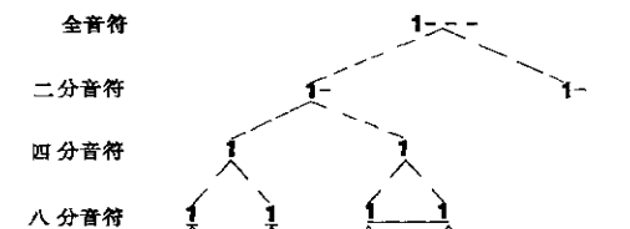
\includegraphics[width=1\textwidth]{yinfu.png}
\end{figure}
\subsection{音符和频率的关系}
       乐曲的十二平均律规定:每2 个八度音(如简谱中的中音1与高音1)之间的频率相差一倍。在2个八度音之间,又可分为12个半音,每2个半音的频率比为。另外,简谱中的低音6的频率为440Hz,音符7到1之间、3到4之间为半音,其余为全音。可计算出简谱中从低音1至高音7之间每个音符的频率:
\begin{figure}[H]
  \centering
  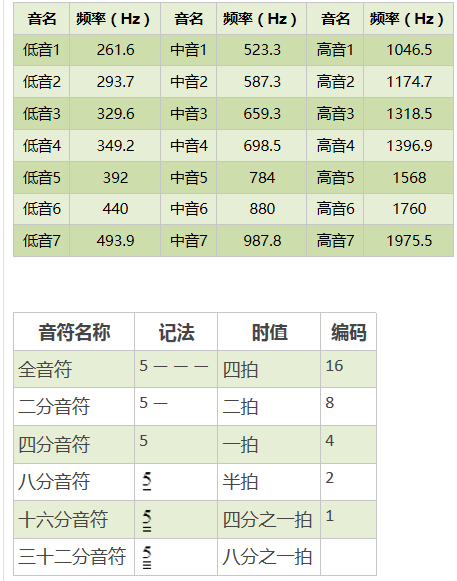
\includegraphics[width=1\textwidth]{frequency.png}
\end{figure}
\subsection{拍控制节奏}
\begin{figure}[H]
  \centering
  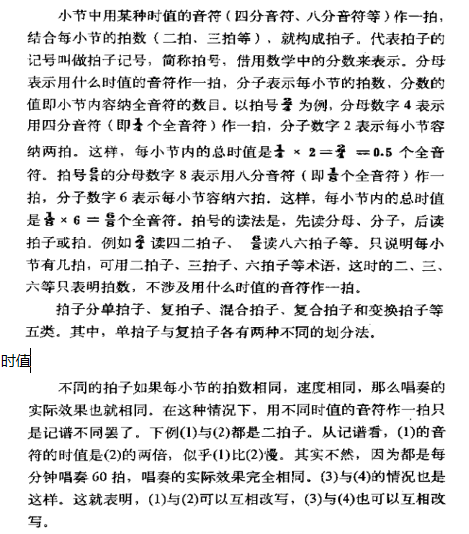
\includegraphics[width=1\textwidth]{pai.png}
\end{figure}

\subsection{发音原理}
通过控制蜂鸣器震动的频率,来产生不同的音调,同时控制此音符的发音时间,达到产生乐曲的效果
通过自己将乐谱数据输入,得到verilog代码。 为了更便捷,我用了python来产生,乐谱即代码见附录。
\section{设备外设}
时钟(50MHz )、拨动开关(2个, ,选择歌曲,复用用)、八段码(3个)用来显示高中低音符,蜂鸣器播放音乐

\section{实验设计}
\subsection{模块划分}
\subsection{拍控制节奏}
\begin{figure}[p]
  \centering
  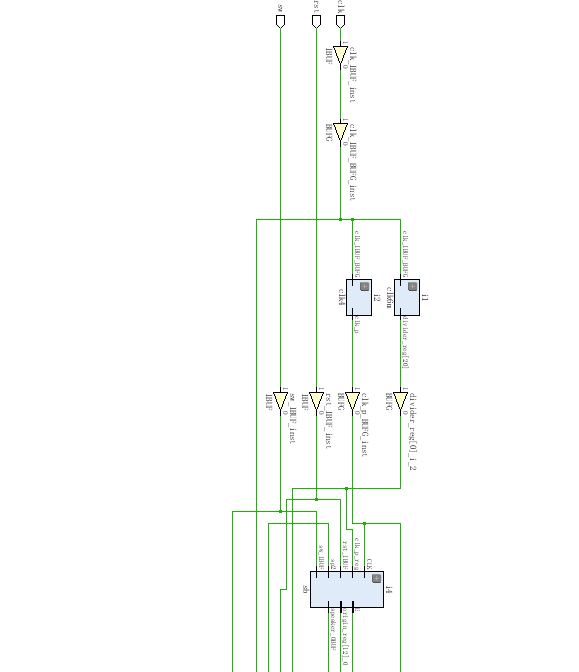
\includegraphics[width=1\textwidth]{m1.png}
\end{figure}
\begin{figure}[p]
  \centering
  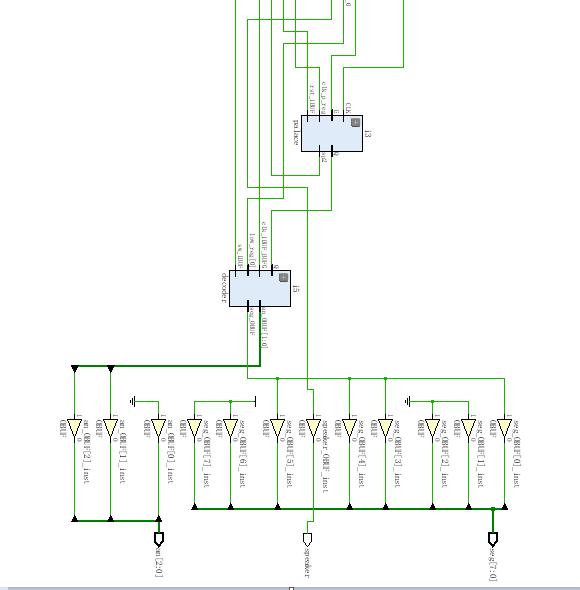
\includegraphics[width=1\textwidth]{m2.png}
\end{figure}
  sb,palace分别为两首乐曲的模块,  mux,为选择模块,clk4, 分频产生4hz的时钟,clk6m,也是分频作用,decoder产生数码管数字

\section{附录}

\subsection{简谱}

\begin{figure}[H]
  \centering

  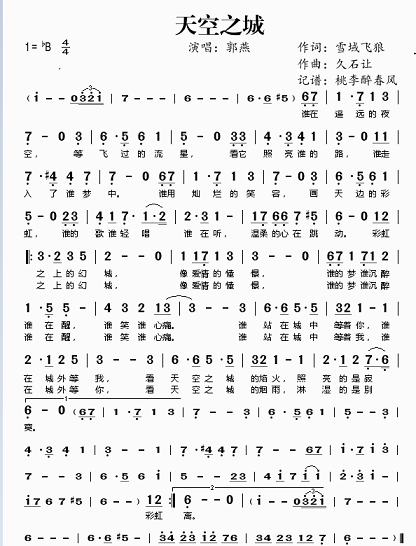
\includegraphics[width=1\textwidth]{sky.png}
\end{figure}

\begin{figure}[H]
  \centering

  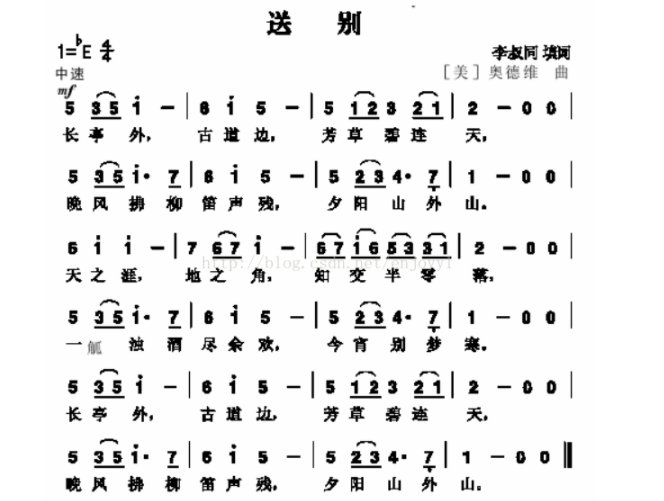
\includegraphics[width=1\textwidth]{sb.png}
\end{figure}


\end{figure}
\subsection{python代码}
\begin{verbatim}
def fgen(fileName='skypalace.txt',base=1): # base是以八分音符为基准,持续的节拍
    li = []
    ct=0
    fmt='{} :{{high,med,low}}=12\'h{};\n'
    # use {} to change the meaning of {} ,namely  {{}}
    with open(fileName,'r') as f:
        #a=1,2,3 低中高音  ,b=1--7 音符,c为节拍,
        for line in f:
            a,b,c=line.strip().split(' ')
            c=int(c)
            b=str(int(b)*base)
            if a=='3':b=b+'00'  
            elif a=='2': b='0'+b+'0'
            elif a=='1':b='00'+b   
            else:b='000'    #休止符
            if b=='000':
                li.append(fmt.format(ct,b))
                ct+=1
                continue
            for i in range(c):
                li.append(fmt.format(ct,b))
                ct+=1
        with open('verilog_2_'+fileName,'w') as tar:
            tar.write(''.join(li))
    return li
\end{verbatim}


\subsection{verilog代码}
\begin{verbatim}
//分频模块  6mhz 
module clk6m    (
input clk,
input rst_n,
output o_clk
);

parameter WIDTH = 4;
parameter N     = 8;

reg [WIDTH-1:0] cnt_p;// 上升沿计数单位
reg [WIDTH-1:0] cnt_n;// 下降沿计数单位
reg             clk_p;// 上升沿时钟
reg             clk_n;// 下降沿时钟

assign o_clk = (N == 1) ? clk :
               (N[0])   ? (clk_p | clk_n) : (clk_p);//其中N==1是判断不分频,N[0]是判断是奇数还是偶数,若为1则是奇数分频,若是偶数则是偶数分频。
        
always@(posedge clk or negedge rst_n) begin
if (!rst_n)
    cnt_p <= 0;
else if (cnt_p == (N-1))
    cnt_p <= 0;
else
    cnt_p <= cnt_p + 1;
end

always@(posedge clk or negedge rst_n) begin
if (!rst_n) 
    clk_p <= 1;//此处设置为0也是可以的,这个没有硬性的要求,不管是取0还是取1结果都是正确的。
else if (cnt_p < (N>>1))/*N整体向右移动一位,最高位补零,其实就是N/2,不过在计算奇数的时候有很明显的优越性*/
    clk_p <= 1;
else
    clk_p <= 0;    
end

always@(negedge clk or negedge rst_n) begin
if (!rst_n)
    cnt_n <= 0;
else if (cnt_n == (N-1))
    cnt_n <= 0;
else
    cnt_n <= cnt_n + 1;
end

always@(negedge clk or negedge rst_n) begin
if (!rst_n)
    clk_n <= 1;
else if (cnt_n < (N>>1))
    clk_n <= 1;
else
    clk_n <= 0;
end

endmodule

//分频模块  4hz 
module clk4    (
input clk,
input rst_n,
output o_clk
);

parameter WIDTH = 35;
parameter N     = 125_00_000;

reg [WIDTH-1:0] cnt_p;// 上升沿计数单位
reg [WIDTH-1:0] cnt_n;// 下降沿计数单位
reg             clk_p;// 上升沿时钟
reg             clk_n;// 下降沿时钟

assign o_clk = (N == 1) ? clk :
               (N[0])   ? (clk_p | clk_n) : (clk_p);//其中N==1是判断不分频,N[0]是判断是奇数还是偶数,若为1则是奇数分频,若是偶数则是偶数分频。
        
always@(posedge clk or negedge rst_n) begin
if (!rst_n)
    cnt_p <= 0;
else if (cnt_p == (N-1))
    cnt_p <= 0;
else
    cnt_p <= cnt_p + 1;
end

always@(posedge clk or negedge rst_n) begin
if (!rst_n) 
    clk_p <= 1;//此处设置为0也是可以的,这个没有硬性的要求,不管是取0还是取1结果都是正确的。
else if (cnt_p < (N>>1))/*N整体向右移动一位,最高位补零,其实就是N/2,不过在计算奇数的时候有很明显的优越性*/
    clk_p <= 1;
else
    clk_p <= 0;    
end

always@(negedge clk or negedge rst_n) begin
if (!rst_n)
    cnt_n <= 0;
else if (cnt_n == (N-1))
    cnt_n <= 0;
else
    cnt_n <= cnt_n + 1;
end

always@(negedge clk or negedge rst_n) begin
if (!rst_n)
    clk_n <= 1;
else if (cnt_n < (N>>1))
    clk_n <= 1;
else
    clk_n <= 0;
end

endmodule
//切换歌曲的选择模块
module mux(
    input clk,sw,sp1,sp2,
    input [11:0] data1,data2,
    output [11:0] data,
    output  sp
    );
    assign sp= (sw==1) ? sp1:sp2,
            data= (sw==1) ? data1:data2;
endmodule

//天空之城
module palace(clk_6MHz,clk_4Hz,rst,speaker,high,med,low); 
input clk_6MHz, clk_4Hz,rst; 
output speaker; 
output[3:0] high,med,low;
reg[3:0] high,med,low; 
reg[25:0] divider,origin; 
reg[10:0] counter; 
reg speaker; 
wire carry; 
 
assign carry=(divider==16383); 
 
always @(posedge clk_6MHz) 
begin   if(carry)  divider=origin; 
else    divider=divider+1; 
end 
 
always @(posedge carry) 
  begin 
speaker=~speaker;         //2 分频产生方波信号 
  end 
 
always @(posedge clk_4Hz) 
    begin 
  case({high,med,low})         //分频比预置 
  12'h001:origin=5506;
  12'h002:origin=6412;
  'b000000000011: origin=7281;
  12'h004:origin=8069; 
  'b000000000101: origin=8730; 
  'b000000000110: origin=9565; 
  'b000000000111: origin=10310; 
  'b000000010000: origin=10647; 
  'b000000100000: origin=11272; 
  'b000000110000: origin=11831;
  12'h040:origin = 12218; 
  'b000001010000: origin=12556; 
  'b000001100000: origin=12974; 
  12'h070:origin=13211;
  12'h100:origin = 13438;
  12'h200:origin = 13672;
  12'h300:origin = 13834;
  12'h400: origin=14000;
  12'h500:origin = 14241;
  12'h600:origin = 14400;
  12'h700:origin = 14600;
  'b000000000000: origin=16383;
  endcase 
    end 
 
always @(posedge clk_4Hz,posedge rst)
    if(rst) counter<=0;
    else
  begin 
if(counter==242)  counter=0;          //计时,以实现循环演奏 
else       counter=counter+1; 
case(counter)              

0 :{high,med,low}=12'h006;

1 :{high,med,low}=12'h007;

2 :{high,med,low}=12'h010;

3 :{high,med,low}=12'h010;

4 :{high,med,low}=12'h010;

5 :{high,med,low}=12'h007;

6 :{high,med,low}=12'h010;

7 :{high,med,low}=12'h010;

8 :{high,med,low}=12'h030;

9 :{high,med,low}=12'h030;

10 :{high,med,low}=12'h007;

11 :{high,med,low}=12'h007;

12 :{high,med,low}=12'h007;

13 :{high,med,low}=12'h007;

14 :{high,med,low}=12'h000;

15 :{high,med,low}=12'h003;

16 :{high,med,low}=12'h003;

17 :{high,med,low}=12'h006;

18 :{high,med,low}=12'h006;

19 :{high,med,low}=12'h006;

20 :{high,med,low}=12'h005;

21 :{high,med,low}=12'h006;

22 :{high,med,low}=12'h006;

23 :{high,med,low}=12'h006;

24 :{high,med,low}=12'h100;

25 :{high,med,low}=12'h100;

26 :{high,med,low}=12'h100;

27 :{high,med,low}=12'h050;

28 :{high,med,low}=12'h050;

29 :{high,med,low}=12'h050;

30 :{high,med,low}=12'h050;

31 :{high,med,low}=12'h000;

32 :{high,med,low}=12'h003;

33 :{high,med,low}=12'h003;

34 :{high,med,low}=12'h004;

35 :{high,med,low}=12'h004;

36 :{high,med,low}=12'h004;

37 :{high,med,low}=12'h003;

38 :{high,med,low}=12'h004;

39 :{high,med,low}=12'h010;

40 :{high,med,low}=12'h010;

41 :{high,med,low}=12'h003;

42 :{high,med,low}=12'h003;

43 :{high,med,low}=12'h003;

44 :{high,med,low}=12'h003;

45 :{high,med,low}=12'h000;

46 :{high,med,low}=12'h010;

47 :{high,med,low}=12'h010;

48 :{high,med,low}=12'h007;

49 :{high,med,low}=12'h007;

50 :{high,med,low}=12'h007;

51 :{high,med,low}=12'h004;

52 :{high,med,low}=12'h004;

53 :{high,med,low}=12'h004;

54 :{high,med,low}=12'h007;

55 :{high,med,low}=12'h007;

56 :{high,med,low}=12'h007;

57 :{high,med,low}=12'h007;

58 :{high,med,low}=12'h007;

59 :{high,med,low}=12'h000;

60 :{high,med,low}=12'h006;

61 :{high,med,low}=12'h007;

62 :{high,med,low}=12'h010;

63 :{high,med,low}=12'h010;

64 :{high,med,low}=12'h010;

65 :{high,med,low}=12'h007;

66 :{high,med,low}=12'h010;

67 :{high,med,low}=12'h010;

68 :{high,med,low}=12'h030;

69 :{high,med,low}=12'h030;

70 :{high,med,low}=12'h007;

71 :{high,med,low}=12'h007;

72 :{high,med,low}=12'h007;

73 :{high,med,low}=12'h000;

74 :{high,med,low}=12'h003;

75 :{high,med,low}=12'h003;

76 :{high,med,low}=12'h006;

77 :{high,med,low}=12'h006;

78 :{high,med,low}=12'h006;

79 :{high,med,low}=12'h005;

80 :{high,med,low}=12'h006;

81 :{high,med,low}=12'h006;

82 :{high,med,low}=12'h010;

83 :{high,med,low}=12'h010;

84 :{high,med,low}=12'h005;

85 :{high,med,low}=12'h005;

86 :{high,med,low}=12'h005;

87 :{high,med,low}=12'h005;

88 :{high,med,low}=12'h000;

89 :{high,med,low}=12'h002;

90 :{high,med,low}=12'h003;

91 :{high,med,low}=12'h004;

92 :{high,med,low}=12'h004;

93 :{high,med,low}=12'h010;

94 :{high,med,low}=12'h007;

95 :{high,med,low}=12'h007;

96 :{high,med,low}=12'h007;

97 :{high,med,low}=12'h010;

98 :{high,med,low}=12'h010;

99 :{high,med,low}=12'h020;

100 :{high,med,low}=12'h020;

101 :{high,med,low}=12'h020;

102 :{high,med,low}=12'h030;

103 :{high,med,low}=12'h010;

104 :{high,med,low}=12'h010;

105 :{high,med,low}=12'h010;

106 :{high,med,low}=12'h010;

107 :{high,med,low}=12'h010;

108 :{high,med,low}=12'h007;

109 :{high,med,low}=12'h006;

110 :{high,med,low}=12'h006;

111 :{high,med,low}=12'h007;

112 :{high,med,low}=12'h007;

113 :{high,med,low}=12'h005;

114 :{high,med,low}=12'h005;

115 :{high,med,low}=12'h006;

116 :{high,med,low}=12'h006;

117 :{high,med,low}=12'h006;

118 :{high,med,low}=12'h006;

119 :{high,med,low}=12'h000;

120 :{high,med,low}=12'h010;

121 :{high,med,low}=12'h020;

122 :{high,med,low}=12'h030;

123 :{high,med,low}=12'h030;

124 :{high,med,low}=12'h030;

125 :{high,med,low}=12'h020;

126 :{high,med,low}=12'h030;

127 :{high,med,low}=12'h030;

128 :{high,med,low}=12'h050;

129 :{high,med,low}=12'h050;

130 :{high,med,low}=12'h020;

131 :{high,med,low}=12'h020;

132 :{high,med,low}=12'h020;

133 :{high,med,low}=12'h020;

134 :{high,med,low}=12'h020;

135 :{high,med,low}=12'h020;

136 :{high,med,low}=12'h000;

137 :{high,med,low}=12'h010;

138 :{high,med,low}=12'h010;

139 :{high,med,low}=12'h010;

140 :{high,med,low}=12'h007;

141 :{high,med,low}=12'h010;

142 :{high,med,low}=12'h010;

143 :{high,med,low}=12'h030;

144 :{high,med,low}=12'h030;

145 :{high,med,low}=12'h030;

146 :{high,med,low}=12'h030;

147 :{high,med,low}=12'h030;

148 :{high,med,low}=12'h030;

149 :{high,med,low}=12'h030;

150 :{high,med,low}=12'h030;

151 :{high,med,low}=12'h000;

152 :{high,med,low}=12'h006;

153 :{high,med,low}=12'h007;

154 :{high,med,low}=12'h010;

155 :{high,med,low}=12'h010;

156 :{high,med,low}=12'h007;

157 :{high,med,low}=12'h010;

158 :{high,med,low}=12'h020;

159 :{high,med,low}=12'h020;

160 :{high,med,low}=12'h010;

161 :{high,med,low}=12'h010;

162 :{high,med,low}=12'h010;

163 :{high,med,low}=12'h005;

164 :{high,med,low}=12'h005;

165 :{high,med,low}=12'h005;

166 :{high,med,low}=12'h005;

167 :{high,med,low}=12'h040;

168 :{high,med,low}=12'h040;

169 :{high,med,low}=12'h030;

170 :{high,med,low}=12'h030;

171 :{high,med,low}=12'h002;

172 :{high,med,low}=12'h002;

173 :{high,med,low}=12'h010;

174 :{high,med,low}=12'h030;

175 :{high,med,low}=12'h030;

176 :{high,med,low}=12'h030;

177 :{high,med,low}=12'h030;

178 :{high,med,low}=12'h030;

179 :{high,med,low}=12'h030;

180 :{high,med,low}=12'h030;

181 :{high,med,low}=12'h030;

182 :{high,med,low}=12'h030;

183 :{high,med,low}=12'h060;

184 :{high,med,low}=12'h060;

185 :{high,med,low}=12'h060;

186 :{high,med,low}=12'h060;

187 :{high,med,low}=12'h050;

188 :{high,med,low}=12'h050;

189 :{high,med,low}=12'h050;

190 :{high,med,low}=12'h050;

191 :{high,med,low}=12'h030;

192 :{high,med,low}=12'h020;

193 :{high,med,low}=12'h010;

194 :{high,med,low}=12'h010;

195 :{high,med,low}=12'h010;

196 :{high,med,low}=12'h010;

197 :{high,med,low}=12'h010;

198 :{high,med,low}=12'h010;

199 :{high,med,low}=12'h020;

200 :{high,med,low}=12'h020;

201 :{high,med,low}=12'h020;

202 :{high,med,low}=12'h010;

203 :{high,med,low}=12'h020;

204 :{high,med,low}=12'h020;

205 :{high,med,low}=12'h050;

206 :{high,med,low}=12'h050;

207 :{high,med,low}=12'h030;

208 :{high,med,low}=12'h030;

209 :{high,med,low}=12'h030;

210 :{high,med,low}=12'h030;

211 :{high,med,low}=12'h030;

212 :{high,med,low}=12'h030;

213 :{high,med,low}=12'h030;

214 :{high,med,low}=12'h030;

215 :{high,med,low}=12'h060;

216 :{high,med,low}=12'h060;

217 :{high,med,low}=12'h060;

218 :{high,med,low}=12'h060;

219 :{high,med,low}=12'h050;

220 :{high,med,low}=12'h050;

221 :{high,med,low}=12'h050;

222 :{high,med,low}=12'h050;

223 :{high,med,low}=12'h030;

224 :{high,med,low}=12'h020;

225 :{high,med,low}=12'h010;

226 :{high,med,low}=12'h010;

227 :{high,med,low}=12'h010;

228 :{high,med,low}=12'h010;

229 :{high,med,low}=12'h010;

230 :{high,med,low}=12'h010;

231 :{high,med,low}=12'h020;

232 :{high,med,low}=12'h020;

233 :{high,med,low}=12'h020;

234 :{high,med,low}=12'h010;

235 :{high,med,low}=12'h020;

236 :{high,med,low}=12'h020;

237 :{high,med,low}=12'h007;

238 :{high,med,low}=12'h007;

239 :{high,med,low}=12'h006;

240 :{high,med,low}=12'h006;

241 :{high,med,low}=12'h006;

242 :{high,med,low}=12'h006;
endcase
end 
endmodule 


//送别

module sb(clk_6MHz,clk_4Hz,rst,speaker,high,med,low); 
input clk_6MHz, clk_4Hz,rst; 
output speaker; 
output[3:0] high,med,low;
reg[3:0] high,med,low; 
reg[25:0] divider,origin; 
reg[10:0] counter; 
reg speaker; 
wire carry; 
 
assign carry=(divider==16383); 
 
always @(posedge clk_6MHz)  if(rst) divider<=0;else
begin   if(carry)  divider=origin; 
else    divider=divider+1; 
end 
 
always @(posedge carry) 
  begin 
speaker=~speaker;         //2 分频产生方波信号 
  end 
 
always @(posedge clk_4Hz) 
  begin 
  case({high,med,low})         //分频比预置 
  12'h001:origin=5506;
  12'h002:origin=6412;
  'b000000000011: origin=7281;
  12'h004:origin=8069; 
  'b000000000101: origin=8730; 
  'b000000000110: origin=9565; 
  'b000000000111: origin=10310; 
  'b000000010000: origin=10647; 
  'b000000100000: origin=11272; 
  'b000000110000: origin=11831;
  12'h040:origin = 12218; 
  'b000001010000: origin=12556; 
  'b000001100000: origin=12974; 
  12'h070:origin=13211;
  12'h100:origin = 13438;
  12'h200:origin = 13672;
  12'h300:origin = 13834;
  12'h400: origin=14000;
  12'h500:origin = 14241;
  12'h600:origin = 14400;
  12'h700:origin = 14600;
  'b000000000000: origin=16383;
  endcase 
  end 
 
always @(posedge clk_4Hz,posedge rst)
    if(rst) counter<=0;
    else
  begin 
if(counter==179)  counter=0;          //计时,以实现循环演奏 
else       counter=counter+1; 
case(counter)              
0 :{high,med,low}=12'h050;

1 :{high,med,low}=12'h050;

2 :{high,med,low}=12'h030;

3 :{high,med,low}=12'h050;

4 :{high,med,low}=12'h100;

5 :{high,med,low}=12'h100;

6 :{high,med,low}=12'h100;

7 :{high,med,low}=12'h100;

8 :{high,med,low}=12'h060;

9 :{high,med,low}=12'h060;

10 :{high,med,low}=12'h100;

11 :{high,med,low}=12'h100;

12 :{high,med,low}=12'h050;

13 :{high,med,low}=12'h050;

14 :{high,med,low}=12'h050;

15 :{high,med,low}=12'h050;

16 :{high,med,low}=12'h050;

17 :{high,med,low}=12'h050;

18 :{high,med,low}=12'h010;

19 :{high,med,low}=12'h020;

20 :{high,med,low}=12'h030;

21 :{high,med,low}=12'h030;

22 :{high,med,low}=12'h020;

23 :{high,med,low}=12'h010;

24 :{high,med,low}=12'h020;

25 :{high,med,low}=12'h020;

26 :{high,med,low}=12'h020;

27 :{high,med,low}=12'h020;

28 :{high,med,low}=12'h000;

29 :{high,med,low}=12'h000;

30 :{high,med,low}=12'h050;

31 :{high,med,low}=12'h050;

32 :{high,med,low}=12'h030;

33 :{high,med,low}=12'h050;

34 :{high,med,low}=12'h100;

35 :{high,med,low}=12'h100;

36 :{high,med,low}=12'h100;

37 :{high,med,low}=12'h070;

38 :{high,med,low}=12'h060;

39 :{high,med,low}=12'h060;

40 :{high,med,low}=12'h100;

41 :{high,med,low}=12'h100;

42 :{high,med,low}=12'h050;

43 :{high,med,low}=12'h050;

44 :{high,med,low}=12'h050;

45 :{high,med,low}=12'h050;

46 :{high,med,low}=12'h050;

47 :{high,med,low}=12'h050;

48 :{high,med,low}=12'h020;

49 :{high,med,low}=12'h030;

50 :{high,med,low}=12'h040;

51 :{high,med,low}=12'h040;

52 :{high,med,low}=12'h040;

53 :{high,med,low}=12'h007;

54 :{high,med,low}=12'h010;

55 :{high,med,low}=12'h010;

56 :{high,med,low}=12'h010;

57 :{high,med,low}=12'h010;

58 :{high,med,low}=12'h000;

59 :{high,med,low}=12'h000;

60 :{high,med,low}=12'h050;

61 :{high,med,low}=12'h050;

62 :{high,med,low}=12'h100;

63 :{high,med,low}=12'h100;

64 :{high,med,low}=12'h100;

65 :{high,med,low}=12'h100;

66 :{high,med,low}=12'h100;

67 :{high,med,low}=12'h100;

68 :{high,med,low}=12'h070;

69 :{high,med,low}=12'h070;

70 :{high,med,low}=12'h060;

71 :{high,med,low}=12'h070;

72 :{high,med,low}=12'h100;

73 :{high,med,low}=12'h100;

74 :{high,med,low}=12'h100;

75 :{high,med,low}=12'h100;

76 :{high,med,low}=12'h050;

77 :{high,med,low}=12'h070;

78 :{high,med,low}=12'h100;

79 :{high,med,low}=12'h060;

80 :{high,med,low}=12'h050;

81 :{high,med,low}=12'h030;

82 :{high,med,low}=12'h030;

83 :{high,med,low}=12'h010;

84 :{high,med,low}=12'h020;

85 :{high,med,low}=12'h020;

86 :{high,med,low}=12'h020;

87 :{high,med,low}=12'h020;

88 :{high,med,low}=12'h000;

89 :{high,med,low}=12'h000;

90 :{high,med,low}=12'h050;

91 :{high,med,low}=12'h050;

92 :{high,med,low}=12'h030;

93 :{high,med,low}=12'h050;

94 :{high,med,low}=12'h100;

95 :{high,med,low}=12'h100;

96 :{high,med,low}=12'h100;

97 :{high,med,low}=12'h070;

98 :{high,med,low}=12'h060;

99 :{high,med,low}=12'h060;

100 :{high,med,low}=12'h100;

101 :{high,med,low}=12'h100;

102 :{high,med,low}=12'h050;

103 :{high,med,low}=12'h050;

104 :{high,med,low}=12'h050;

105 :{high,med,low}=12'h050;

106 :{high,med,low}=12'h050;

107 :{high,med,low}=12'h050;

108 :{high,med,low}=12'h020;

109 :{high,med,low}=12'h030;

110 :{high,med,low}=12'h040;

111 :{high,med,low}=12'h040;

112 :{high,med,low}=12'h040;

113 :{high,med,low}=12'h007;

114 :{high,med,low}=12'h010;

115 :{high,med,low}=12'h010;

116 :{high,med,low}=12'h010;

117 :{high,med,low}=12'h010;

118 :{high,med,low}=12'h000;

119 :{high,med,low}=12'h000;

120 :{high,med,low}=12'h050;

121 :{high,med,low}=12'h050;

122 :{high,med,low}=12'h030;

123 :{high,med,low}=12'h050;

124 :{high,med,low}=12'h100;

125 :{high,med,low}=12'h100;

126 :{high,med,low}=12'h100;

127 :{high,med,low}=12'h100;

128 :{high,med,low}=12'h060;

129 :{high,med,low}=12'h060;

130 :{high,med,low}=12'h100;

131 :{high,med,low}=12'h100;

132 :{high,med,low}=12'h050;

133 :{high,med,low}=12'h050;

134 :{high,med,low}=12'h050;

135 :{high,med,low}=12'h050;

136 :{high,med,low}=12'h050;

137 :{high,med,low}=12'h050;

138 :{high,med,low}=12'h010;

139 :{high,med,low}=12'h020;

140 :{high,med,low}=12'h030;

141 :{high,med,low}=12'h030;

142 :{high,med,low}=12'h020;

143 :{high,med,low}=12'h010;

144 :{high,med,low}=12'h020;

145 :{high,med,low}=12'h020;

146 :{high,med,low}=12'h020;

147 :{high,med,low}=12'h020;

148 :{high,med,low}=12'h000;

149 :{high,med,low}=12'h000;

150 :{high,med,low}=12'h050;

151 :{high,med,low}=12'h050;

152 :{high,med,low}=12'h030;

153 :{high,med,low}=12'h050;

154 :{high,med,low}=12'h100;

155 :{high,med,low}=12'h100;

156 :{high,med,low}=12'h100;

157 :{high,med,low}=12'h070;

158 :{high,med,low}=12'h050;

159 :{high,med,low}=12'h050;

160 :{high,med,low}=12'h100;

161 :{high,med,low}=12'h100;

162 :{high,med,low}=12'h050;

163 :{high,med,low}=12'h050;

164 :{high,med,low}=12'h050;

165 :{high,med,low}=12'h050;

166 :{high,med,low}=12'h050;

167 :{high,med,low}=12'h050;

168 :{high,med,low}=12'h020;

169 :{high,med,low}=12'h030;

170 :{high,med,low}=12'h040;

171 :{high,med,low}=12'h040;

172 :{high,med,low}=12'h040;

173 :{high,med,low}=12'h007;

174 :{high,med,low}=12'h010;

175 :{high,med,low}=12'h010;

176 :{high,med,low}=12'h010;

177 :{high,med,low}=12'h010;

178 :{high,med,low}=12'h000;

179 :{high,med,low}=12'h000;
endcase 
end 
endmodule 

//数码管
module decoder (input clk,input [11:0] in ,output  reg[7:0] out,output  [3:1]AN);
        reg [2:0] an;
        reg [4:1] cur;
        reg [20:1] cnt;
        assign AN = an;
        parameter k=266666;
        always@(posedge clk)
            if(cnt==k)cnt<=0;
            else cnt=cnt+1;
        always@(posedge clk)
            if(an==4&&cnt==k)an<=0;
            else if(cnt==k)an<=an+2;
            else an<=an;
        always@(*)
            case (an)
            0: cur = in[3:0];
            2:cur = in[7:4];
            4:cur = in[11:8];
            endcase
            
        always@(*)
            begin 
                case(cur)
                0:out<=8'b1100_0000;
                1:out<=8'b1111_1001;
                2:out<=8'b1010_0100;
                3:out<=8'b1011_0000;                    
                4:out<=8'b1001_1001;
                5:out<=8'b1001_0010;
                6:out<=8'b1000_0010;
                7:out<=8'b1101_1000;
                8:out<=8'b1000_0000;
                9:out<=8'b1001_0000;
                10:out<=8'b1000_1000;
                11:out<=8'b1000_0011;
                12:out<=8'b1100_0110;
                13:out<=8'b1010_0001;
                14:out<=8'b1000_0110;
                15:out<=8'b1000_1110;
                endcase
            end
endmodule


//顶层模块
module tp(
    input clk,rst,sw,
    output [7:0]seg,
    output [2:0]an,
    output speaker

    );
    wire [3:0]  h1,h2,m1,m2,l1,l2;
    wire [7:0] seg1,seg2;
    wire sp1,sp2;
    wire c4,c6m;
    clk6m i1(clk,1,c6m);
    clk4 i2(clk,1,c4);
    mux  i6(clk,sw,sp1,sp2,{h1,m1,l1},{h2,m2,l2},data,speaker);
    sb  i4(c6m,c4,rst,sp1,h1,m1,l1);
    palace  i3(c6m,c4,rst,sp2,h2,m2,l2);
    decoder i5(clk,data,seg,an);
endmodule

\end{verbatim}



\end{document}